\documentclass[10pt]{article}

\usepackage{spheric}
%%%TITLE
\title{SPH numerical simulation of lift-off by impact of sand particles on flat sand bed}
\date{}

%%AFFILIATIONS
\author[$\relax$]{Zhao Jie}
\author[$\relax$]{Jin A. Fang}
\author[$\relax$]{Maimtimin Geni}
\author[$\relax$]{Ma. Xiaojing}
\affil[$\relax$]{College of Mechanical Engineering, Xinjiang University, Urumqi Xinjiang 830047 China}


\newcommand\blfootnote[1]{%
  \begingroup
  \renewcommand\thefootnote{}\footnote{#1}%
  \addtocounter{footnote}{-1}%
  \endgroup
}
%%DOCUMENT
\begin{document}
\maketitle

%\SelectedTopics{}

%%PLEASE PUT YOUR ABSTRACT HERE
\begin{abstract}
The study of Aeolian processes can offer insights into past and present geographies and climatic conditions. Previous models of the collision between sand particles are complex and require enormous amounts of calculation.In this paper, we use SPH method to simulate the lift-off phenomenon of sand particles in air flows which impact the surface of a grain bed. And the approach in this paper avoids in dealing with large deformation and the complexities of generating grids with complicated shapes and areas.Our study provides a better simulation method for research on the micro-movements of wind-blown sand.

The paper considers atmospheric boundary layer as a two-dimensional space,and use the Boussinesq assumptions to simplify the control equation (Bagnold 1941) ,then, using the SPH method,the whole computational domain is broken down into discrete particles using control equations .These discrete particles are consistent with natural sand particles in terms of shape. Therefore, using the SPH method has particular advantages in processing collision problems of sand particles. We carry out statistical analyses and compare our results with previous studies, and our simulated results show that the collision effect is very important for the take-off of sand particles in wind-blown sand movement and that it dictates the entire process of sand movement. The collision effect of sand particles can stir up several bigger and heavier sand particles. The simulated results demonstrate the micro-collision process more dynamically and precisely.

\begin{figure}[!htb]
\centering
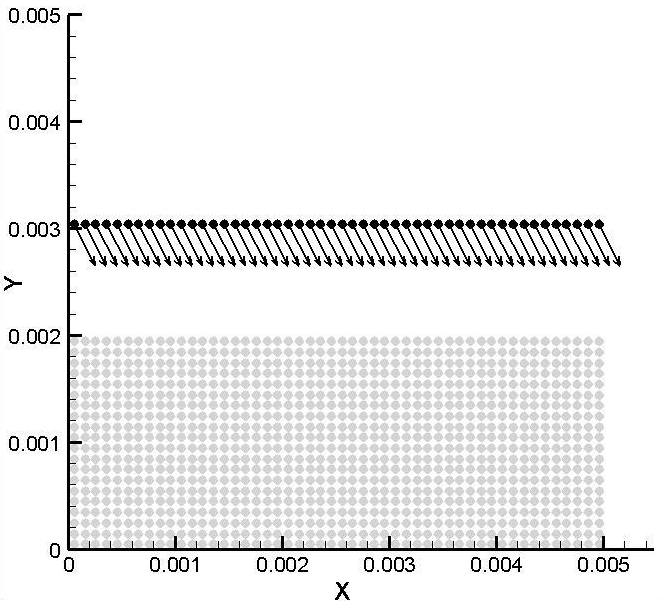
\includegraphics[width=0.32\textwidth]{44-11.png}
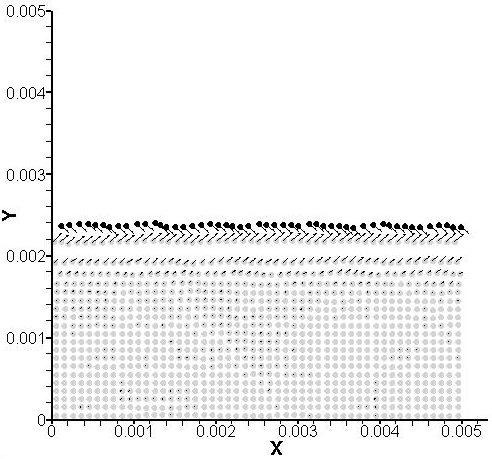
\includegraphics[width=0.32\textwidth]{44-12.png}
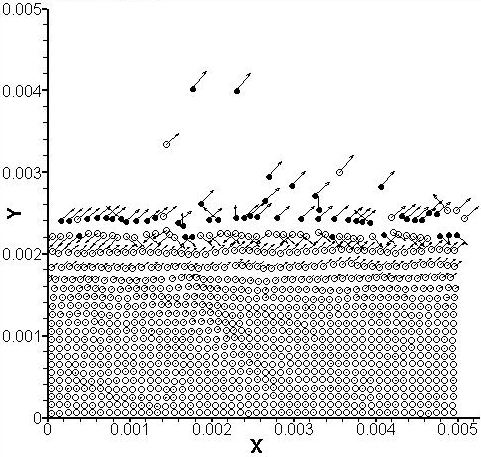
\includegraphics[width=0.32\textwidth]{44-13.png}
\caption{Dynamic process of sand impacting bed surface:initial distribution of sand particles before collision when step is 0(left).Position and velocity of sand particles at step is 4000 (middle).Velocity and direction of sand particles after collision when step is 5000 (right).}\label{fig:44}
\end{figure}

\blfootnote{Project supported by the National Natural Science Foundation of China(Grant No.11662019) and University Scientific Research Plan of Xinjiang Uygur Autonomous Region (Grant No.XJEDU2016S031)}
\end{abstract}


%%THE END OF ABSTRACT

\addbib

\end{document}
